\documentclass[]{beamer}
\usetheme{KUL}
\usepackage{multirow}
\usepackage{multicol}
\usepackage{tikz}
\usepackage{ulem}
\usepackage{siunitx}
\newcommand\itemS{\item[\textbf{\S}]}
\definecolor{darkgreen}{rgb}{0,0.598,0.199}
\usepackage{times} % set font on times new roman
\usepackage{eurosym} % package for Euro sign
\usepackage{lineno}   % package for line numbering
\usepackage{hyperref} % this is for url links
\usepackage{subcaption}  % this package enables one to put several figures next to each other
\usepackage{textcomp}
\usepackage{setspace}
\usepackage{gensymb}

%----------------------------------
% Fill in the essential Information
%----------------------------------

\title[Main title]{Matrix project}
\subtitle{\ldots Artificial Intelligence and Machine Learning}
\author[A.\ rishitha]{Rishitha\\Adithya} % between [] is short name, between {} is long name
\date{\today} % Here you can also just type something, e.g. October 10, 2017
\institute[KU Leuven]{Indian Institute Of Technology Hyderabad}
% ACTUAL PRESENTATION STARTS HERE
%----------------------------------

\begin{document}

% TITEL PAGE	
	{
		\setbeamertemplate{headline}{} %define local, empty header for title page
		\setbeamertemplate{footline}{} %define local, empty footer for title page
		\maketitle
	}
	\addtocounter{framenumber}{-1} % We don't count the title page

% FRAME 1 
\section{}
\begin{frame}{EE1390}
\begin{itemize}
    \item Geometrical form of question
    
\end{itemize}
\begin{kulblock}{Question}
    Find the locus of point of intersection of the straight lines:
\begin{equation}
    tx-2y-3t=0
\end{equation} 
\begin{equation}
    x-2ty+3=0
\end{equation}
\end{kulblock}
\end{frame}

% FRAME 2
\begin{frame}{EE1390}
\begin{itemize}
    \item Matrix transformation of geometrical question
\end{itemize}
Find the locus of point of intersection of straight lines:
\[\begin{bmatrix}
    t&-2
\end{bmatrix}
X=3t\]
\[\begin{bmatrix}
1&-2t
\end{bmatrix}
X=-3\]
\end{frame}

% FRAME 3
\begin{frame}{EE1390}
\begin{itemize}
    \item solution in terms of matrices
\end{itemize}
\[\begin{bmatrix}
t&-2
\end{bmatrix}
X=3t\]
\[\begin{bmatrix}
1&-2t
\end{bmatrix}
X=-3\]
The point of intersection of the above lines is\\\\
\centering
(n_1)^TX=p_1\\
\centering\\
(n_2)^TX=p_2
\end{frame}
\begin{frame}
\[\centering
N^TX=P\]
where
\[N^T=
\begin{bmatrix}
n_1^T&n_2^T
\end{bmatrix}\]
and
\[n_1^T=
\begin{bmatrix}
t&-2
\end{bmatrix}\]
\[n_2^T=
\begin{bmatrix}
1&-2
\end{bmatrix}\]
\[N=
\begin{bmatrix}
t&1\\-2&-2t
\end{bmatrix}\]
We get the point of intersection from\\
\centering
X=(N^-^T)P
\end{frame}
\begin{frame}
\centering
\begin{itemize}
    \item Where
\end{itemize}
det(N^T)=
\[\frac{1}{2-2t^2}\]  
\begin{itemize}
    \item Hence
\end{itemize}
N^-^T=\[\frac{1}{2-2t^2}\]
\begin{bmatrix}
-2t&2\\-1&t
\end{bmatrix}\\\\
And
\[P
\begin{bmatrix}
3t\\-3
\end{bmatrix}\]
\begin{itemize}
    \item Therefore after solving for X ,we get
\end{itemize}
\[X=
\begin{bmatrix}
\frac{3(t^2+1}{t^2-1}\\
\frac{3t}{t^2-1}
\end{bmatrix}\]
\end{frame}
\begin{frame}{figure}
 \frametitle{Locus of the equation}
\begin{figure}
    \centering
    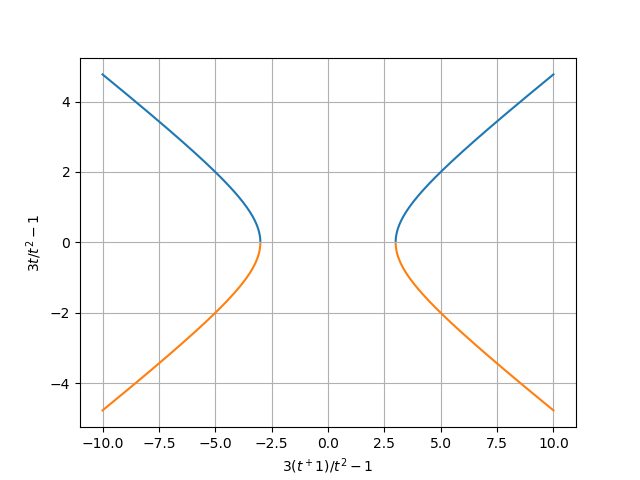
\includegraphics[scale=0.5]{hyp.png}
    \caption{HYPERBOLA}
\end{figure}
\end{frame}
\end{document}